\documentclass[12pt
,headinclude
,headsepline
,bibtotocnumbered
]{scrartcl}
\usepackage[paper=a4paper,left=25mm,right=25mm,top=25mm,bottom=25mm]{geometry} 
\usepackage[utf8]{inputenc}
\usepackage[english]{babel}
\usepackage{fancyvrb}  % Add this line
\usepackage{graphicx}
\usepackage{multirow}
\usepackage{pdfpages}
%\usepackage{wrapfig}
\usepackage{placeins}
\usepackage{float}
\usepackage{flafter}
\usepackage{mathtools}
\usepackage{hyperref}
\usepackage{epstopdf}
\usepackage[miktex]{gnuplottex}
\usepackage[T1]{fontenc}
\usepackage{mhchem}
\usepackage{fancyhdr}
%\setlength{\mathindent}{0pt}
\usepackage{amssymb}
\usepackage[list=true, font=large, labelfont=bf, 
labelformat=brace, position=top]{subcaption}
\setlength{\parindent}{0mm}
\usepackage{listings}
\usepackage{color}

\definecolor{dkgreen}{rgb}{0,0.6,0}
\definecolor{gray}{rgb}{0.5,0.5,0.5}
\definecolor{mauve}{rgb}{0.58,0,0.82}

\lstset{ %
	language=Python,                % the language of the code
	basicstyle=\small\ttfamily,     % the size of the fonts that are used for the code
	numbers=left,                   % where to put the line-numbers
	numberstyle=\tiny\color{gray},  % the style that is used for the line-numbers
	stepnumber=1,                   % the step between two line-numbers. If it's 1, each line will be numbered
	numbersep=5pt,                  % how far the line-numbers are from the code
	backgroundcolor=\color{white},  % choose the background color. You must add \usepackage{color}
	showspaces=false,               % show spaces adding particular underscores
	showstringspaces=false,         % underline spaces within strings
	showtabs=false,                 % show tabs within strings adding particular underscores
	frame=single,                   % adds a frame around the code
	rulecolor=\color{black},        % if not set, the frame-color may be changed on line-breaks within not-black text (e.g. commens (green here))
	tabsize=2,                      % sets default tabsize to 2 spaces
	captionpos=b,                   % sets the caption-position to bottom
	breaklines=true,                % sets automatic line breaking
	breakatwhitespace=true,         % sets if automatic breaks should only happen at whitespace
	title=\lstname,                 % show the filename of files included with \lstinputlisting; also try caption instead of title
	keywordstyle=\color{blue},      % keyword style
	commentstyle=\color{dkgreen},   % comment style
	stringstyle=\color{mauve},      % string literal style
	escapeinside={\%*}{*)},         % if you want to add LaTeX within your code
	morekeywords={*,...}            % if you want to add more keywords to the set
}

\setlength{\parindent}{0mm}

\pagestyle{fancy}
\fancyhf{}
\lhead{Orbit Mechanics\\ Exercise 1: Keplerian Orbits}
\rhead{Hsin-Feng Ho \\03770686}
\rfoot{Page \thepage}	
\begin{document}
\section{Introduction}
In this exercise, we will study the Keplerian orbits in different coordinate systems. The Keplerian obital elements for 5 satellites are given in the table below. The orbital elements are given in the following order: semi-major axis $a$, eccentricity $e$, inclination $i$, right ascension of the ascending node $\Omega$, argument of perigee $\omega$, and perigee passing time $T_0$ on Nov.06,2023.
\begin{table}[H]
\centering
\renewcommand\arraystretch{1.5}
\setlength{\tabcolsep}{5mm}{
\begin{tabular}{|c|c|c|c|c|c|c|}
    \hline
    \textbf{Satellite}& \textbf{a[km]}&\textbf{e}&\textbf{i[deg]}&\textbf{$\boldsymbol{\Omega}$[deg]}&\textbf{$\boldsymbol{\omega}$[deg]}&\textbf{$\boldsymbol{T_0}$[s]}\\\hline
    GOCE&6629&0.004&96.6&210&144&01:00\\\hline
    GPS&26560&0.001&55&30&30&11:00\\\hline
    Molniya&26554&0.7&63&200&270&05:00\\\hline
    GEO&42164&0&0&0&50&00:00\\\hline
    Michibiki&42164&0.075&41&200&270&19:00\\\hline

\end{tabular}
}
\end{table}
\subsection*{Orbit in 2D plane}
In this first task we will calculate the polar coordinates of stellite postion. The Keplerian elements of the semi-major axis and eccentricity are given. These two parameters determine the shape of the orbit. Then we have to calculate the current position of the satellite on this orbit plane with the time of perigee passage, where $\nu=E=M=0$. This allows us to calculate the orbit evolution over time. 
\begin{equation*}
    \boldsymbol{r}_f(r,\nu)=\begin{bmatrix}
        r\cos\nu\\
        r\sin\nu\\
        0
    \end{bmatrix}
    =\begin{bmatrix}
        a\cos E-e\\
        a\sqrt{1-e^2}\sin E\\
        0
    \end{bmatrix}
\end{equation*}
r is the distance from the center of the ellipse to the satellite, and $\nu$ is the true anomaly. The true anomaly is the angle between the perigee and the satellite position. The eccentric anomaly $E$ is the angle between the perigee and the position of the satellite on the ellipse. The eccentric anomaly can be calculated by solving the Kepler equation.
\begin{equation*}
    M=E-e\sin E
\end{equation*}
The mean anomaly $M$ is the angle between the perigee and the position of the satellite on the circle. This is a fictitious angle and it evolves linearly in time. The mean anomaly can be calculated by the following equation.
\begin{equation*}
    M=n(t-T_0)
\end{equation*}
The mean motion $n$ is the angular velocity of the satellite on the orbit. The mean motion can be calculated by the following equation.
\begin{equation*}
    n=\sqrt{\frac{\mu}{a^3}}=\sqrt{\frac{GM}{a^3}}
\end{equation*}
The five satellite orbit in 2D plane are shown in Figure \ref{fig:2D_orbit}. The orbit of GOCE is a circular orbit, and the orbit of GPS is a nearly circular orbit. The orbit of Molniya is a highly eccentric orbit. The orbit of GEO is a circular orbit, and the orbit of Michibiki is a nearly circular orbit.
\begin{figure}[H]
    \centering
    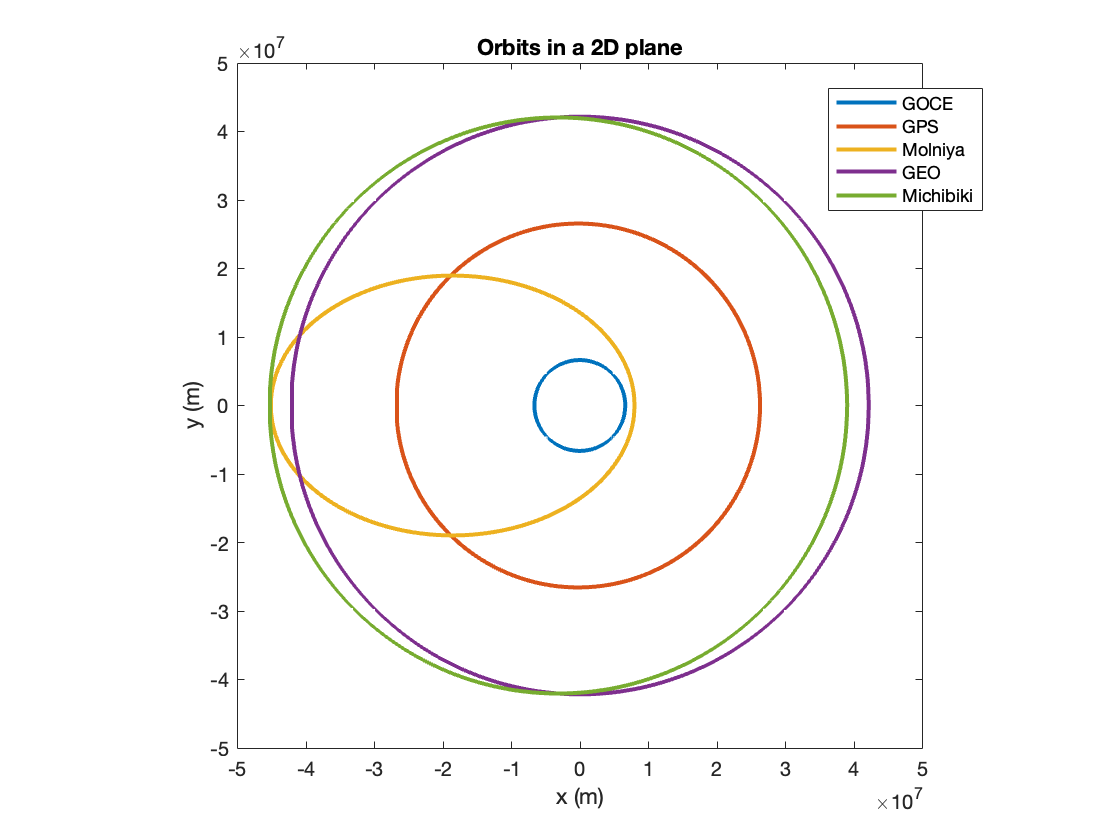
\includegraphics[width=0.8\textwidth]{plots/orb2d.png}
    \caption{2D orbit}
    \label{fig:2D_orbit}
\end{figure}
We also have to plot the mean anomaly $M$, the eccentric anomaly $E$ and the true anomaly $\nu$ over 12 hours for the GPS and Molniya satellite.
\begin{figure}[H]
    \centering
    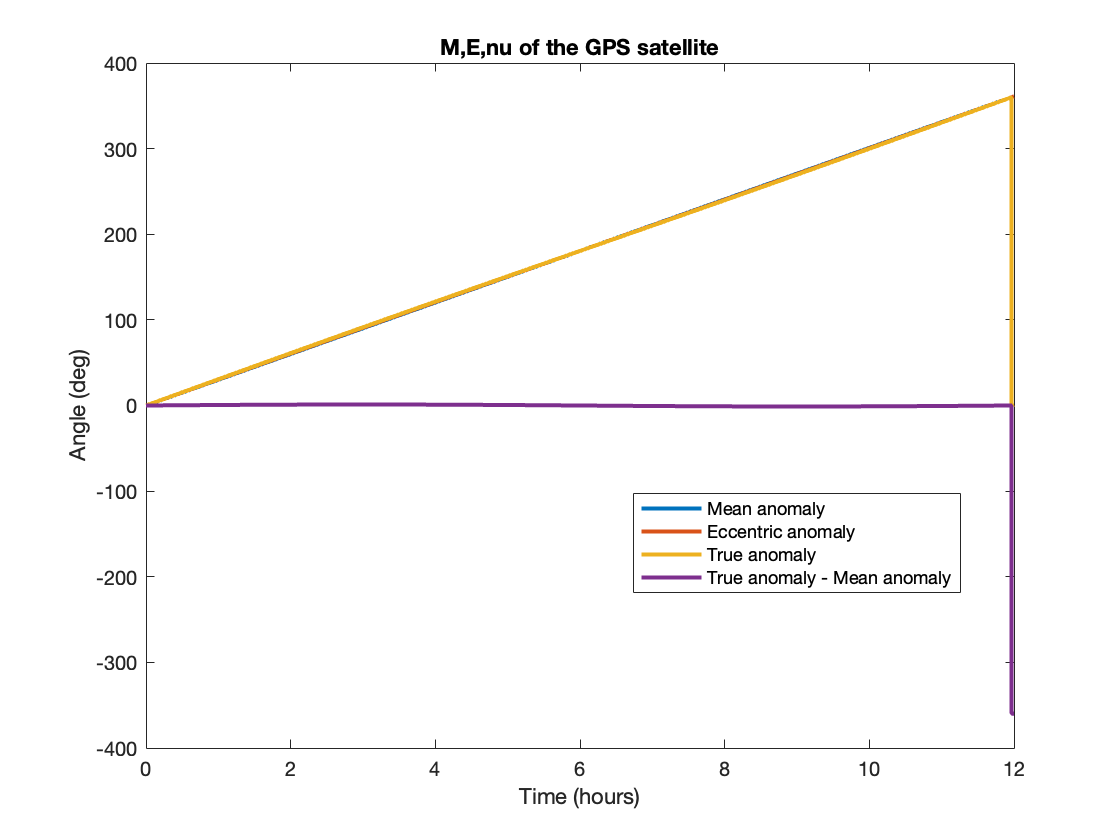
\includegraphics[width=0.8\textwidth]{plots/MG.png}
    \caption{Mean, eccentric and true anomaly of GPS}
    \end{figure}
\begin{figure}[H]
    \centering
    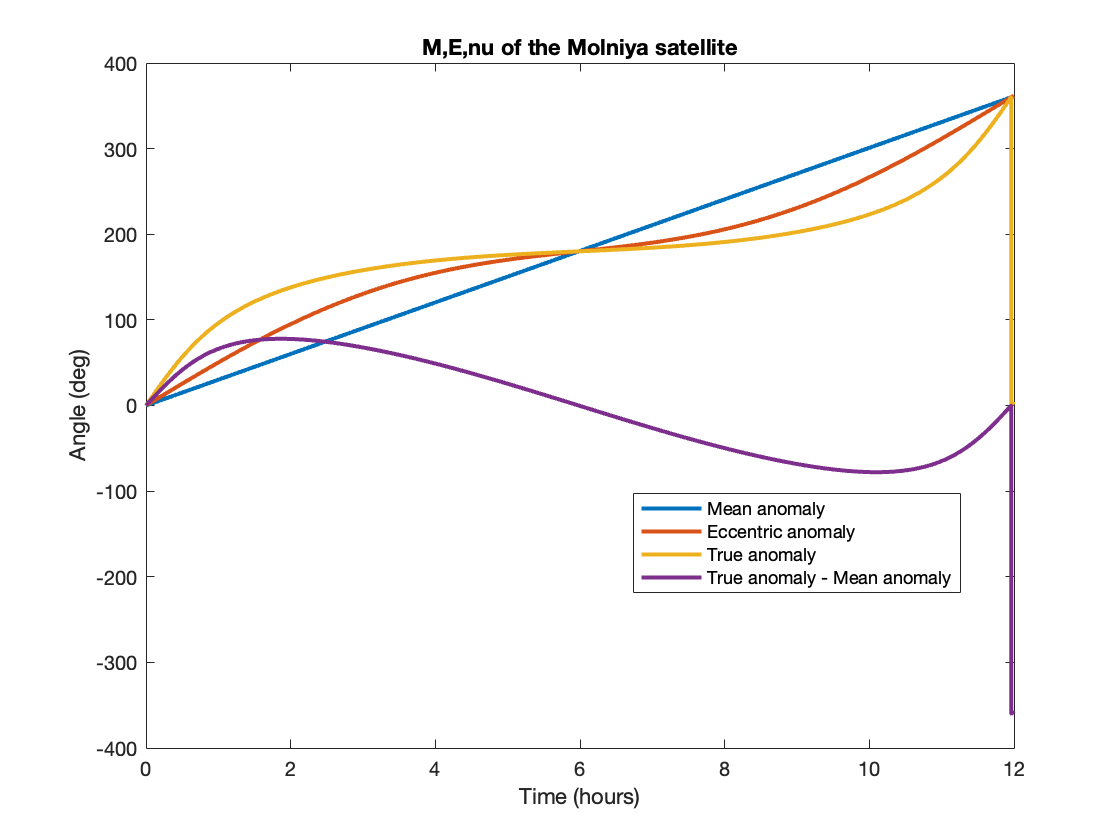
\includegraphics[width=0.8\textwidth]{plots/MM.png}
    \caption{Mean, eccentric and true anomaly of Molniya}
\end{figure}
We can observe that the mean anomaly $M$ is a linear function of time. The orbit of GPS is nearly circular, since the true anomaly $\nu$ increases similar with mean anomaly. On the other hand, the orbit of Molniya is highly eccentric, since the true anomaly $\nu$ increases in a periodic matter. 
\subsection*{Space-fixed inertial system}
In this second task we want to transform the satellite postion and velocity from the perifocal $f$-frame of 2D plane to the cartesian coordinates of 3D space in an inertial space fixed system. 
\begin{align*}
    \boldsymbol{r}_i=\boldsymbol{R}_3(-\Omega)\boldsymbol{R}_1(-i)\boldsymbol{R}_3(-\omega)\boldsymbol{r}_f\\
    \dot{\boldsymbol{r}}_i=\boldsymbol{R}_3(-\Omega)\boldsymbol{R}_1(-i)\boldsymbol{R}_3(-\omega)\dot{\boldsymbol{r}}_f
\end{align*}
After transformation we can plot the 3D orbit and the projection of 3D orbit and velocity. The 3D orbit is shown in Figure \ref{fig:3D_orbit}. The projection of 3D orbit and velocity are shown in Figure \ref{fig:images}. The orbits of GOCE and GPS are nearly circular. The orbit of Molniya is a highly eccentric orbit. The orbit of GEO is a circular orbit, and the orbit of Michibiki is a elliptical orbit. In the velocity plot we see that the velocity of Molniya changes periodicly over time, while the other satellites have only slight changes in velocity. 
\begin{figure}[H]
    \centering
    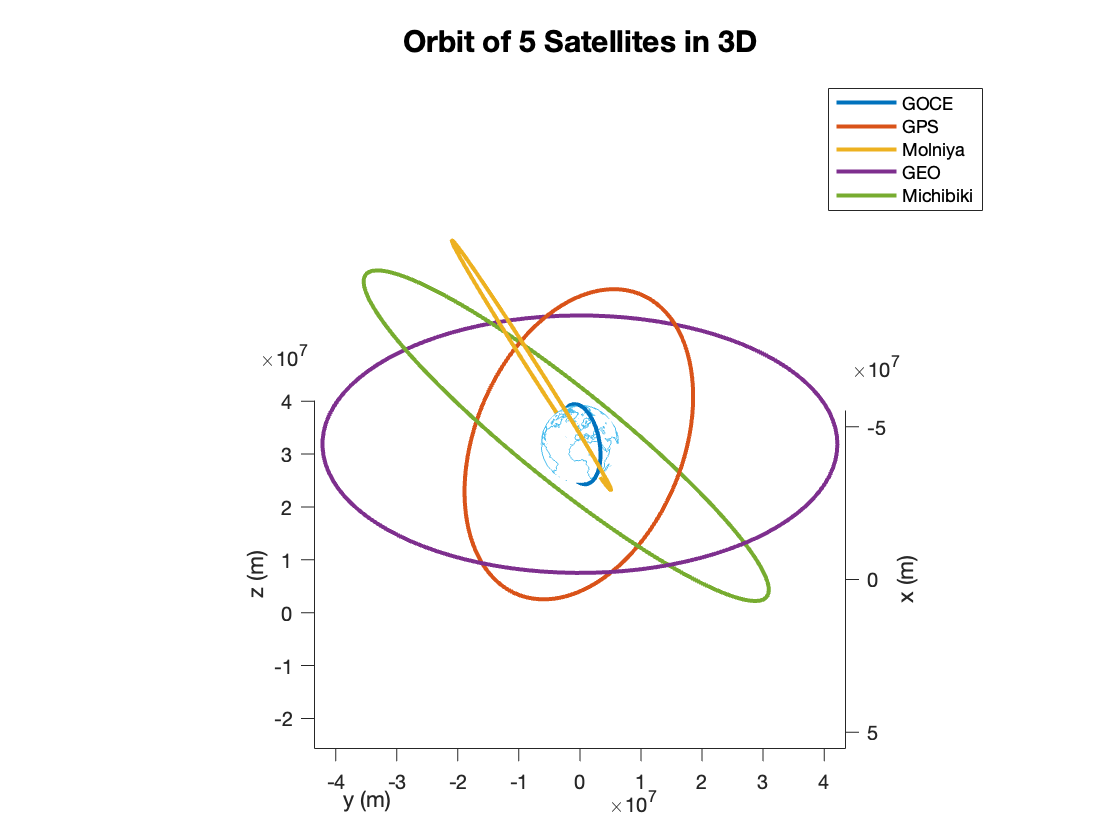
\includegraphics[width=0.65\textwidth]{plots/orb3d.png}
    \caption{3D orbit}
    \label{fig:3D_orbit}
\end{figure}
\begin{figure}[H]
    \centering
    \begin{subfigure}[b]{0.45\textwidth}
        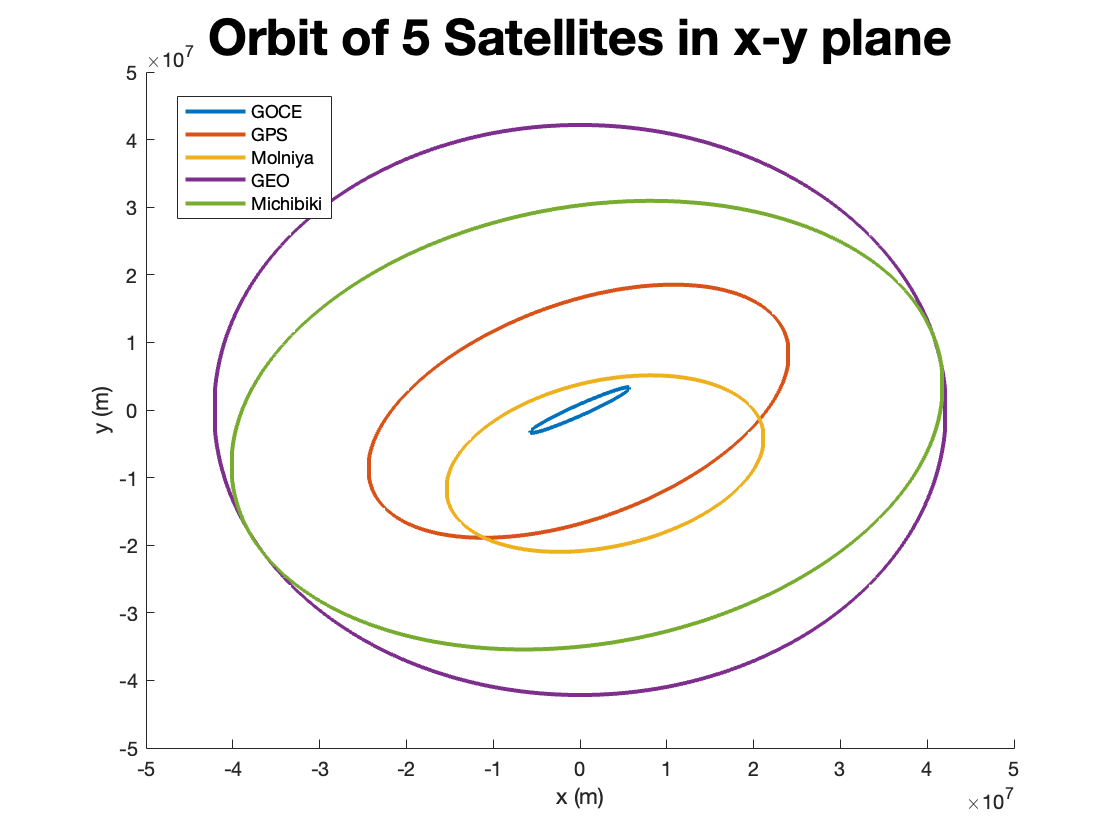
\includegraphics[width=\textwidth]{plots/orbxy.png}
        \label{fig:image1}
    \end{subfigure}
    \begin{subfigure}[b]{0.45\textwidth}
        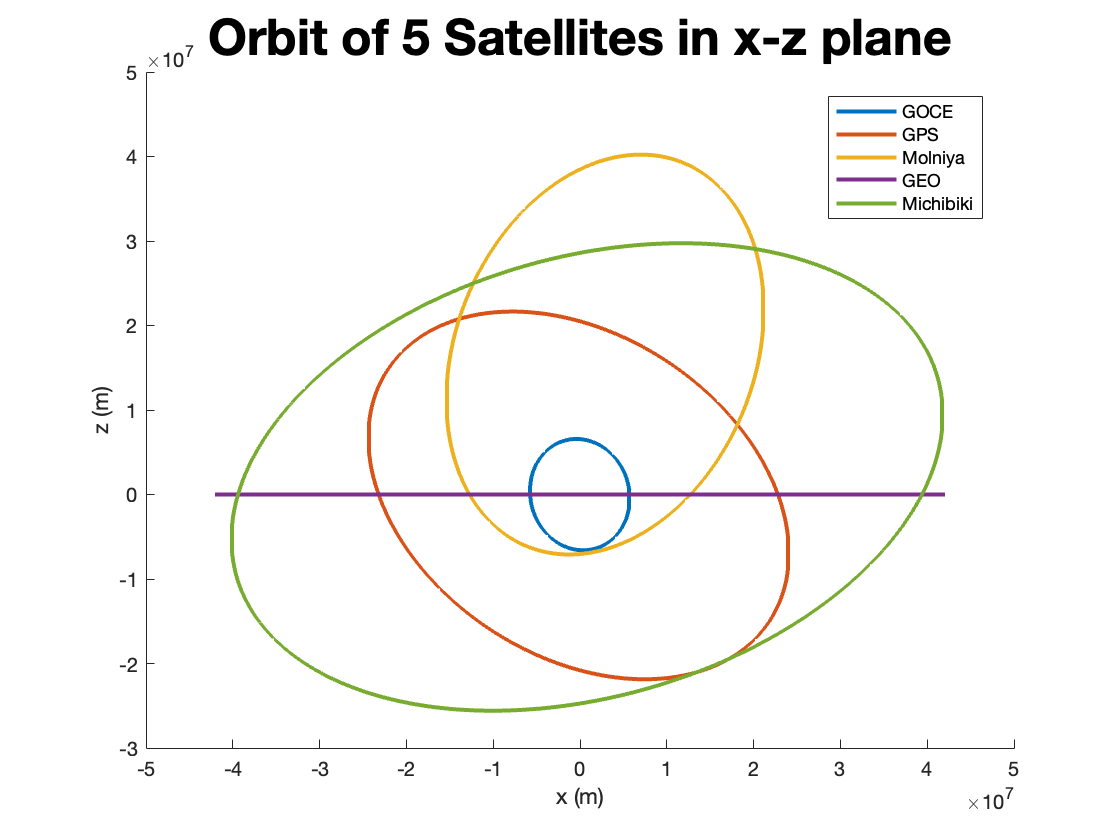
\includegraphics[width=\textwidth]{plots/orbxz.png}
        \label{fig:image2}
    \end{subfigure}
    \begin{subfigure}[b]{0.45\textwidth}
        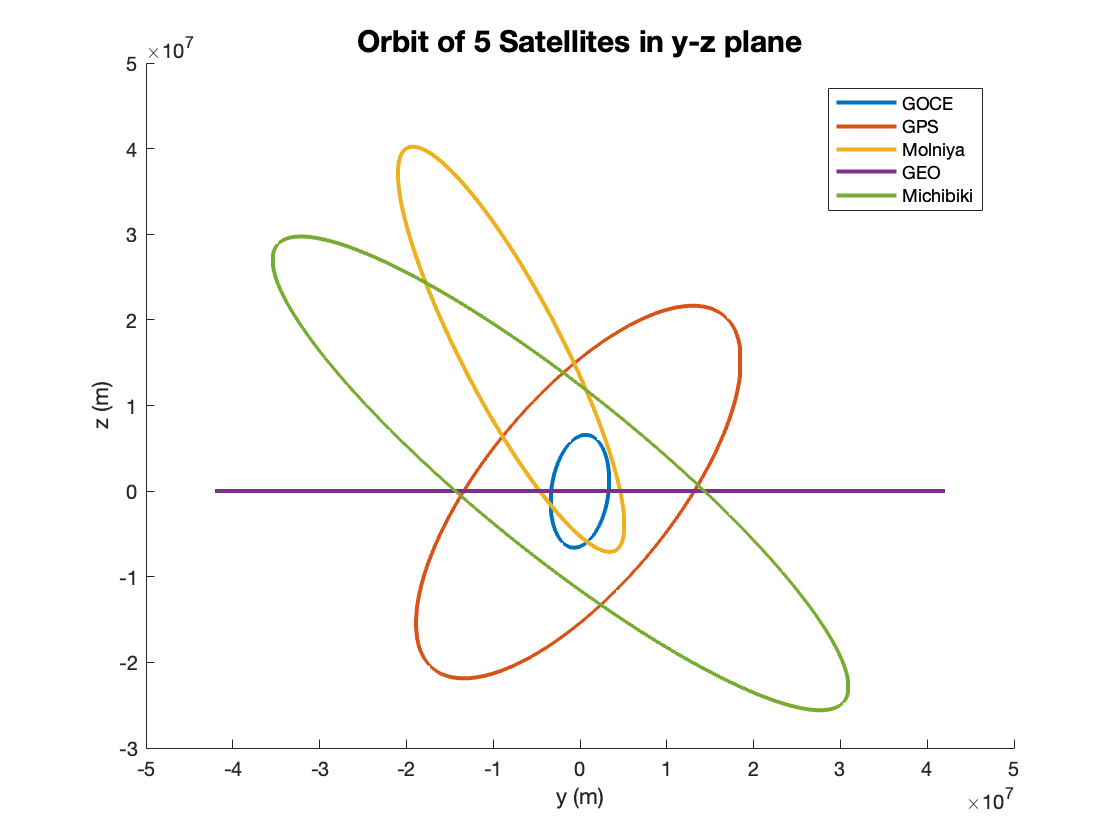
\includegraphics[width=\textwidth]{plots/orbyz.png}
        \label{fig:image3}
    \end{subfigure}
    \begin{subfigure}[b]{0.45\textwidth}
        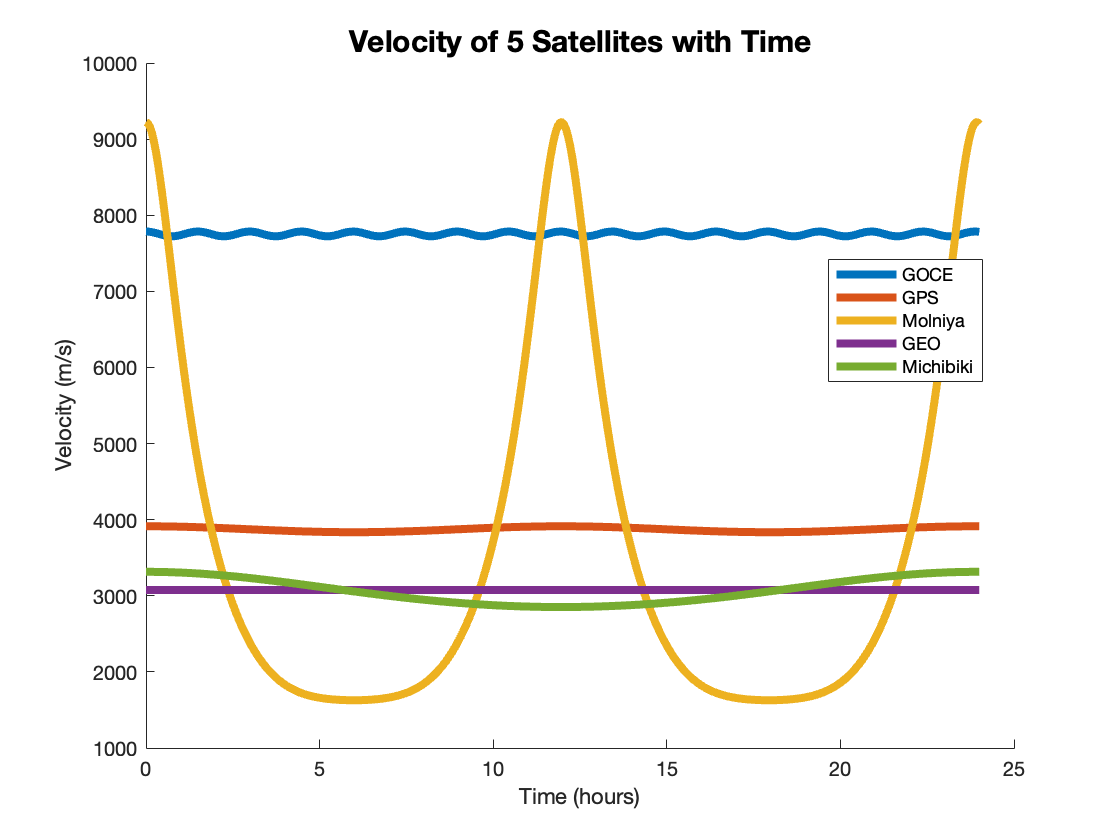
\includegraphics[width=\textwidth]{plots/velocity.png}
        \label{fig:image4}
    \end{subfigure}
    \caption{Projection of 3D orbit and velocity}
    \label{fig:images}
\end{figure}
\section*{Earth-fixed system}
In this task we have to transform the satellite postion and velocity from the cartesian coordinates of 3D space in an inertial space fixed system to the cartesian coordinates of 3D space in an Earth-fixed system. The Earth-fixed system is a rotating system with respect to Earth rotation rate. The transformation can be calculated by the following equation.
\begin{align*}
    \theta&=\dot{\Omega}_Et+\text{sidereal angle}\\
    \boldsymbol{r}_e&=\boldsymbol{R}_3(-\theta)\boldsymbol{r}_i
\end{align*}
which $\dot{\Omega}_E$ is the Earth rotation rate. The Earth rotation rate is calculated by $\frac{2\pi}{86164}$. The sidereal angle is the angle between the Greenwich meridian and the equinox. In this exercise we use a sidereal angle of 3 hours. The satellite position in Earth-fixed system is shown in Figure \ref{fig:earth_fixed}.
\begin{figure}[H]
    \centering
    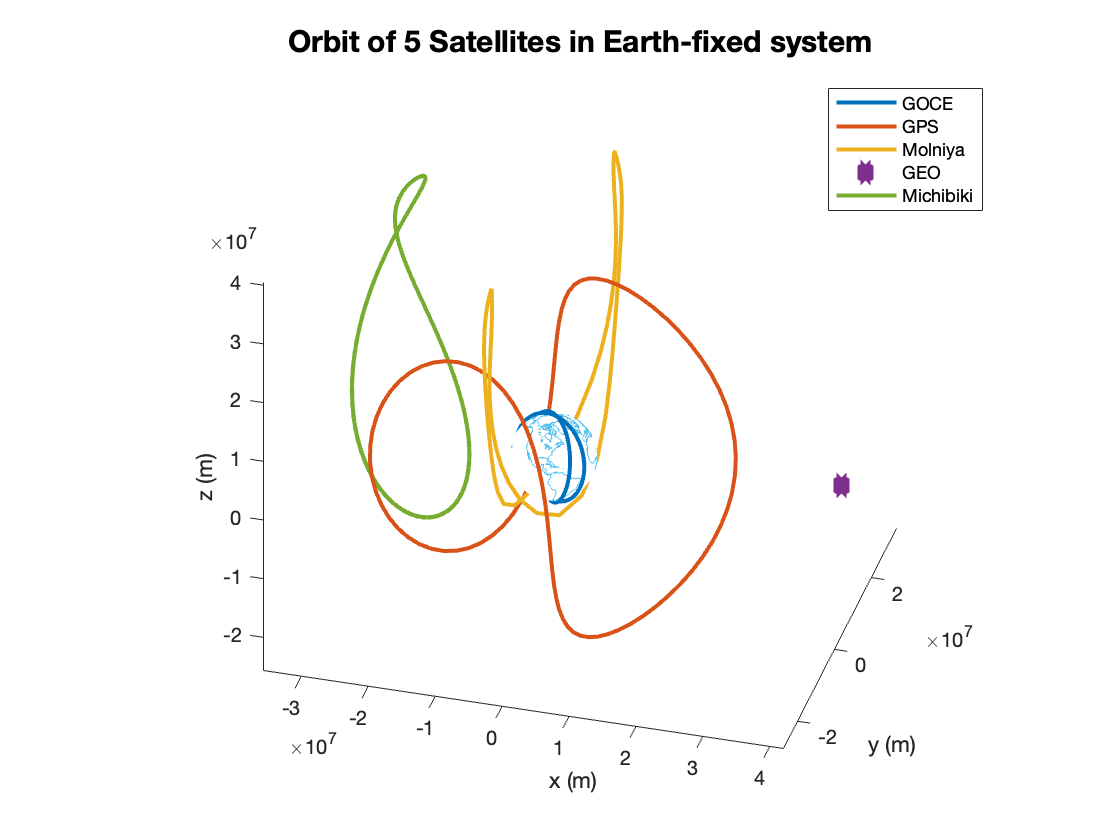
\includegraphics[width=0.7\textwidth]{plots/orbefix.png}
    \caption{Earth-fixed system}
    \label{fig:earth_fixed}
\end{figure}
The satellite ground-tracks on the Earth surface will also be calculated and shown in Figure \ref{fig:ground_track}.
\begin{align*}
    \lambda&=\arctan\left(\frac{y}{x}\right)\\
    \phi&=\arctan\left(\frac{z}{\sqrt{x^2+y^2}}\right)
\end{align*}
After calculation we get the ground-track of the satellites. The GEO satellite stays at the same position on the Earth surface, since the GEO satellite is a geostationary satellite. And the ground track of the Michibiki satellite is a figure of eight.
\begin{figure}[H]
    \centering
    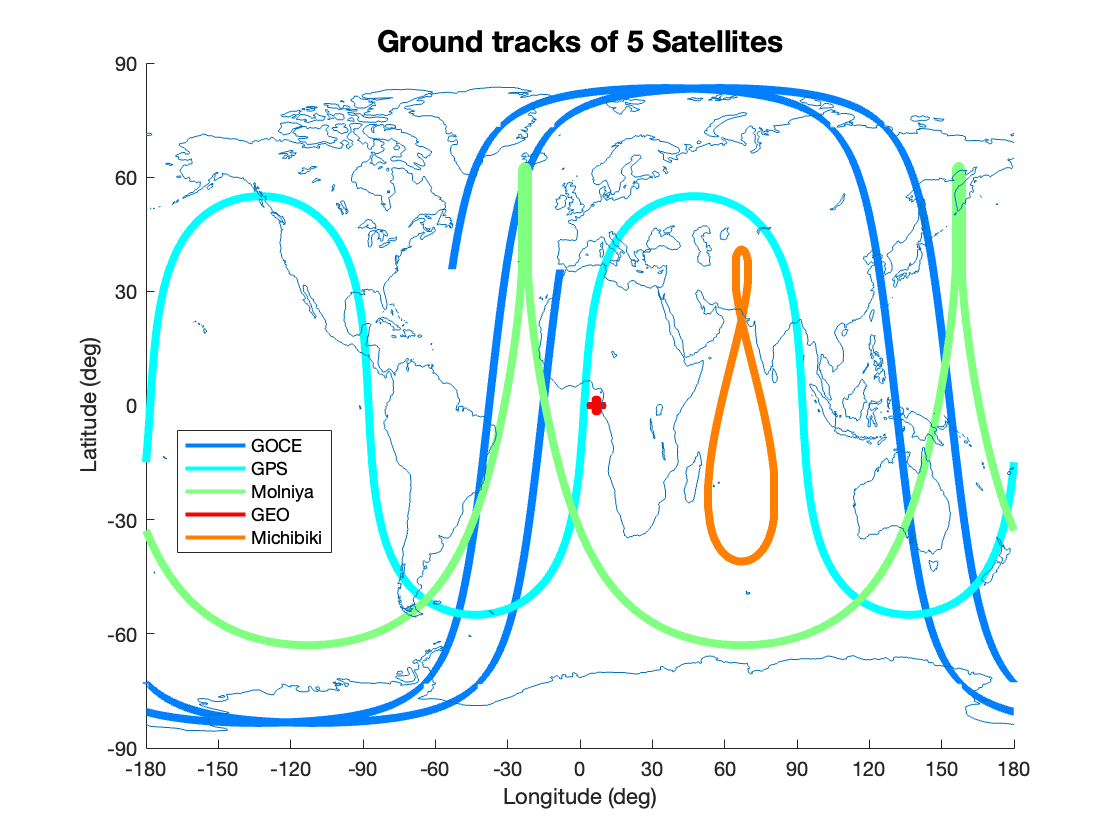
\includegraphics[width=0.7\textwidth]{plots/groundtrack.png}
    \caption{Ground-track}
    \label{fig:ground_track}
\end{figure}
\subsection*{Topocentric system}
The position vector of the station Wettzell is given in the Earth-fixed system: $\boldsymbol{r}_w=(4075.53022, 931.78130, 4801.61819)^T$ km. The position vector of the satellite in the topocentric system is calculated by the following equation.
\begin{align*}
    \boldsymbol{r}_t&=\boldsymbol{r}_e-\boldsymbol{r}_w\\
    \boldsymbol{r}_t&=\boldsymbol{Q}_1\boldsymbol{R}_2(90-\Phi_w)\boldsymbol{R}_3(\lambda_w)\boldsymbol{r}_t\\
    Q_1&=\begin{bmatrix}
        -1&0&0\\
        0&1&0\\
        0&0&1
    \end{bmatrix}
\end{align*}
The $Q_1$ matrix is used to transfrom from right- to left-handed system. \\\\
It's also useful to compute the azimuth and elevation of the satellites in the topocentric system. The azimuth and elevation are calculated by the following equation.
\begin{align*}
    \text{azimuth}&=\arctan\left(\frac{y_t}{x_t}\right)\\
    \text{elevation}&=\arctan\left(\frac{z_t}{\sqrt{x_t^2+y_t^2}}\right)
\end{align*}
And now we can plot the trajectory of the satellites that can be observed by Wettzell. The trajectory of the satellites that can be observed by Wettzell is shown in Figure \ref{fig:topocentric}.
\begin{figure}[H]
    \centering
    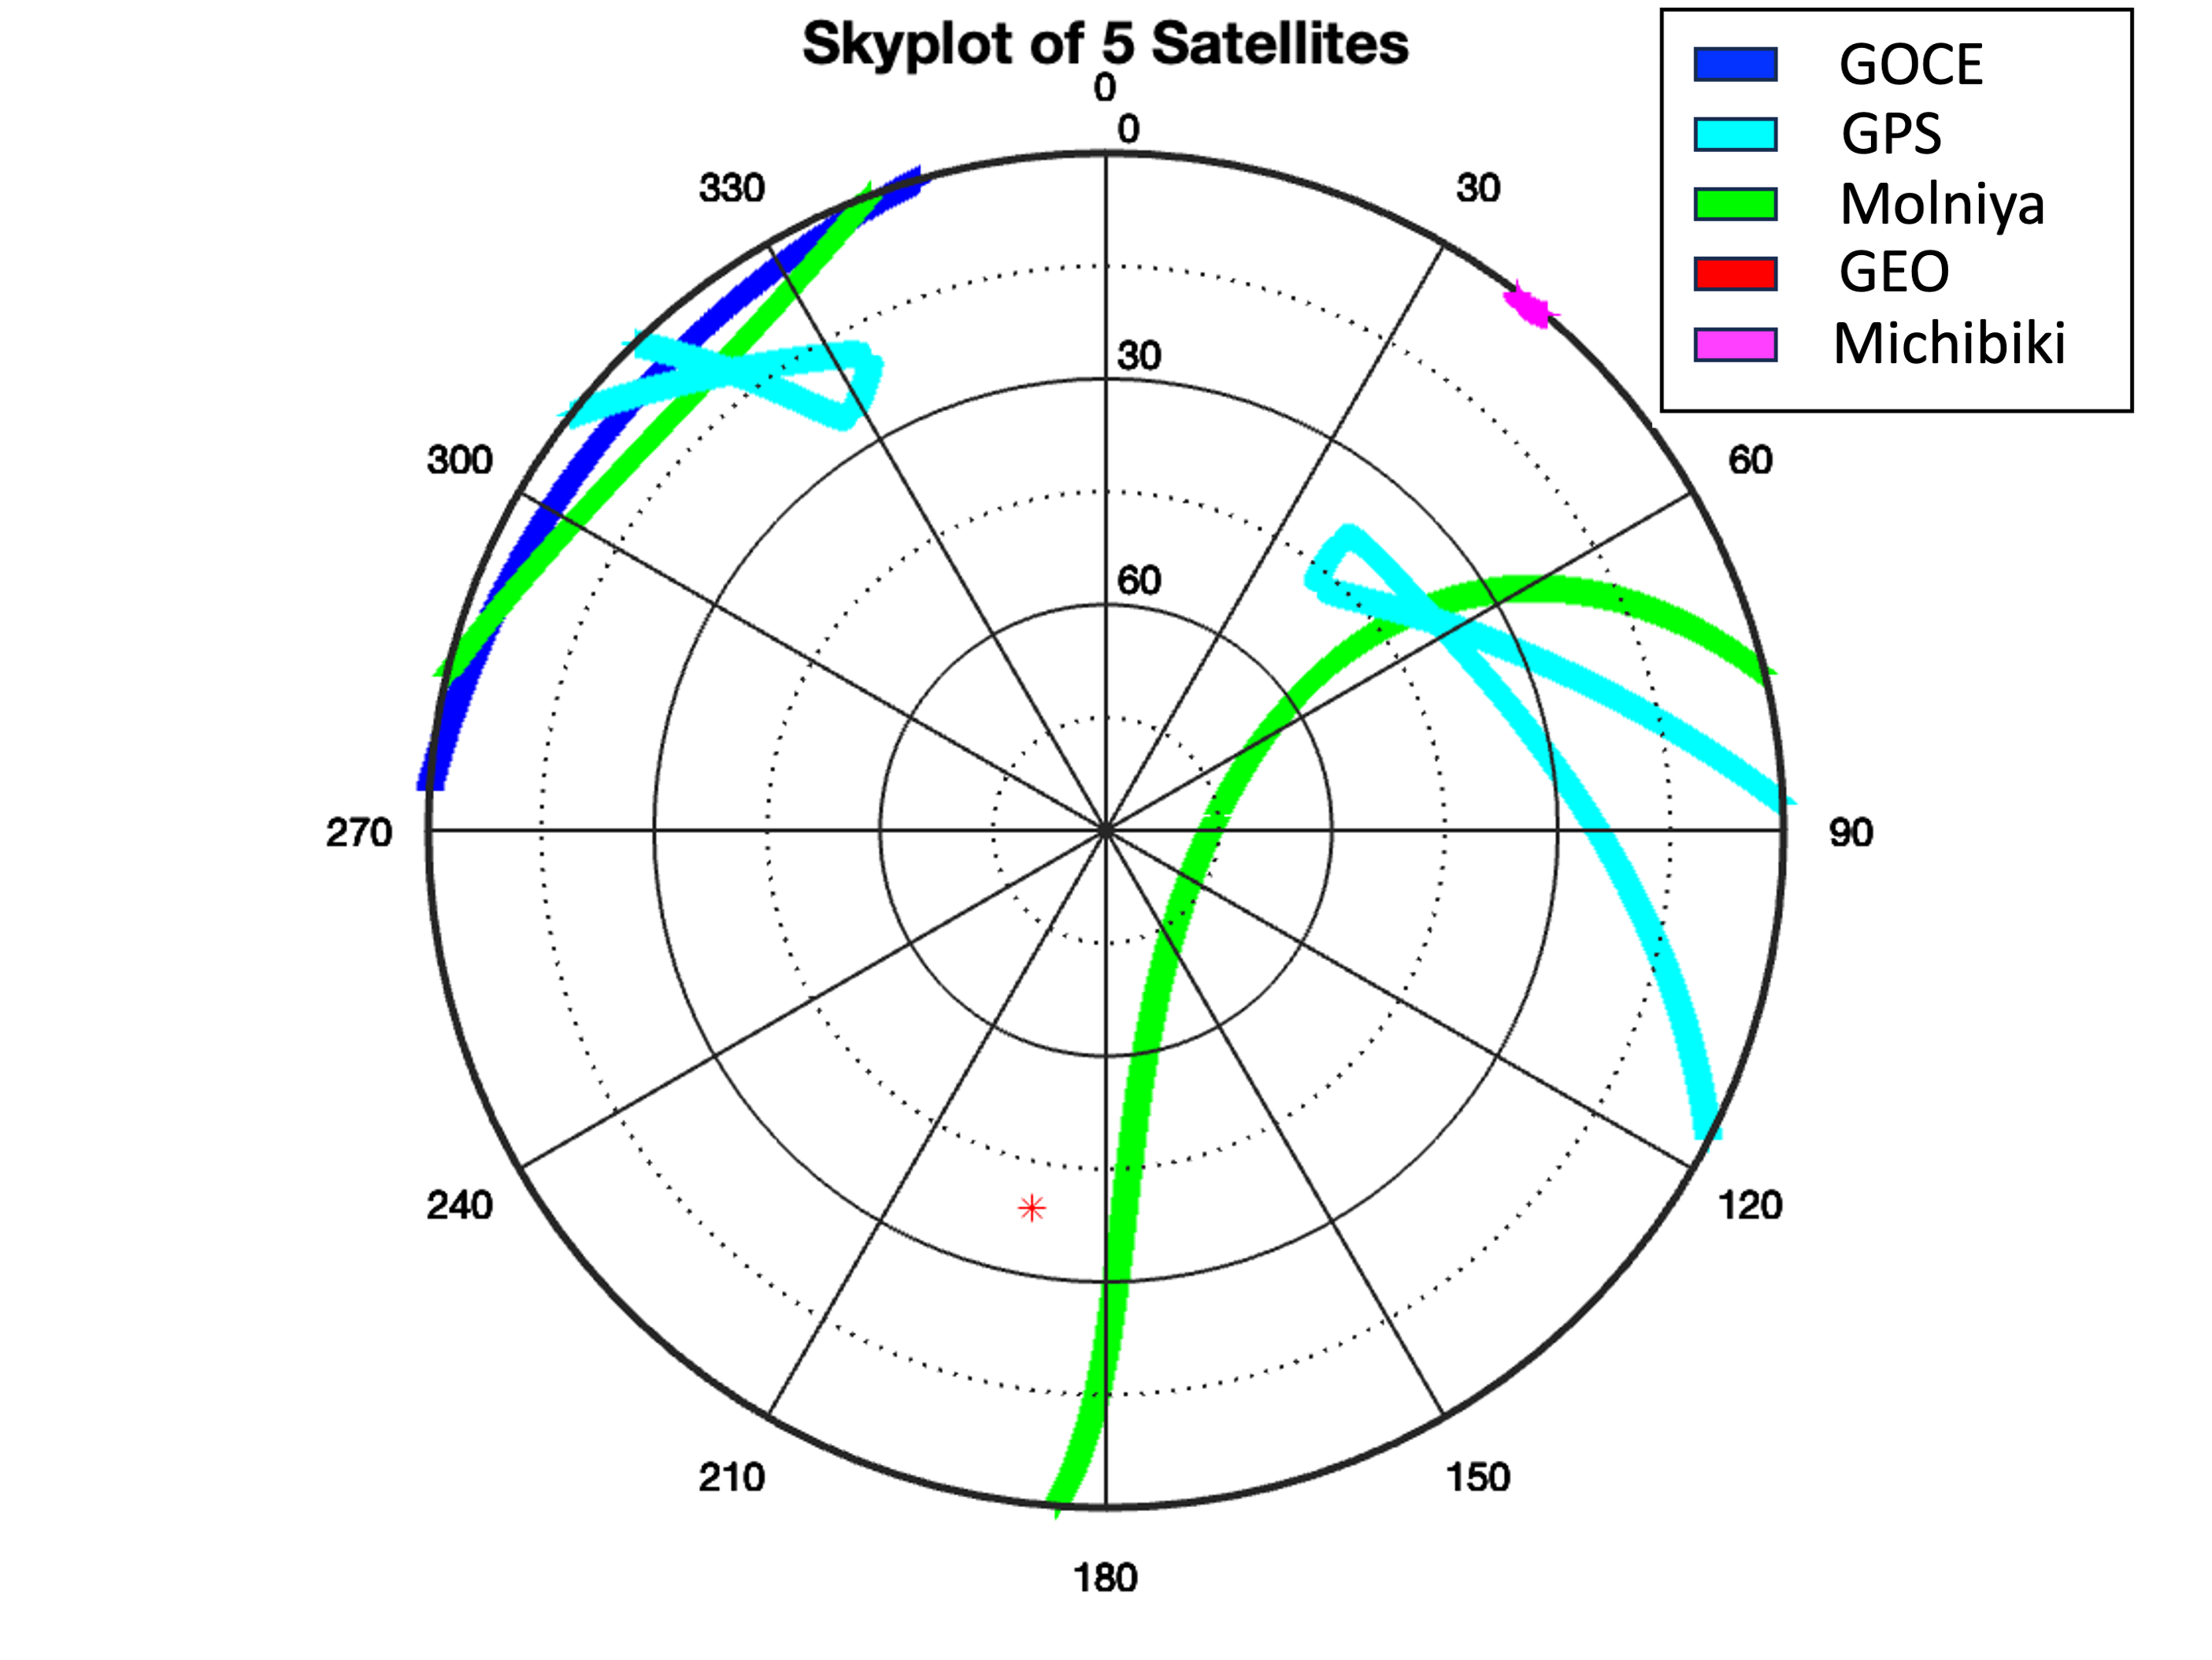
\includegraphics[width=0.7\textwidth]{plots/topocentric.png}
    \caption{Topocentric system}
    \label{fig:topocentric}
\end{figure}
Finally we can calculate the visibility of the satellites at the station Wettzell. The visibility of the satellites at the station Wettzell is shown in Figure \ref{fig:visibility}.
\begin{figure}[H]
    \centering
    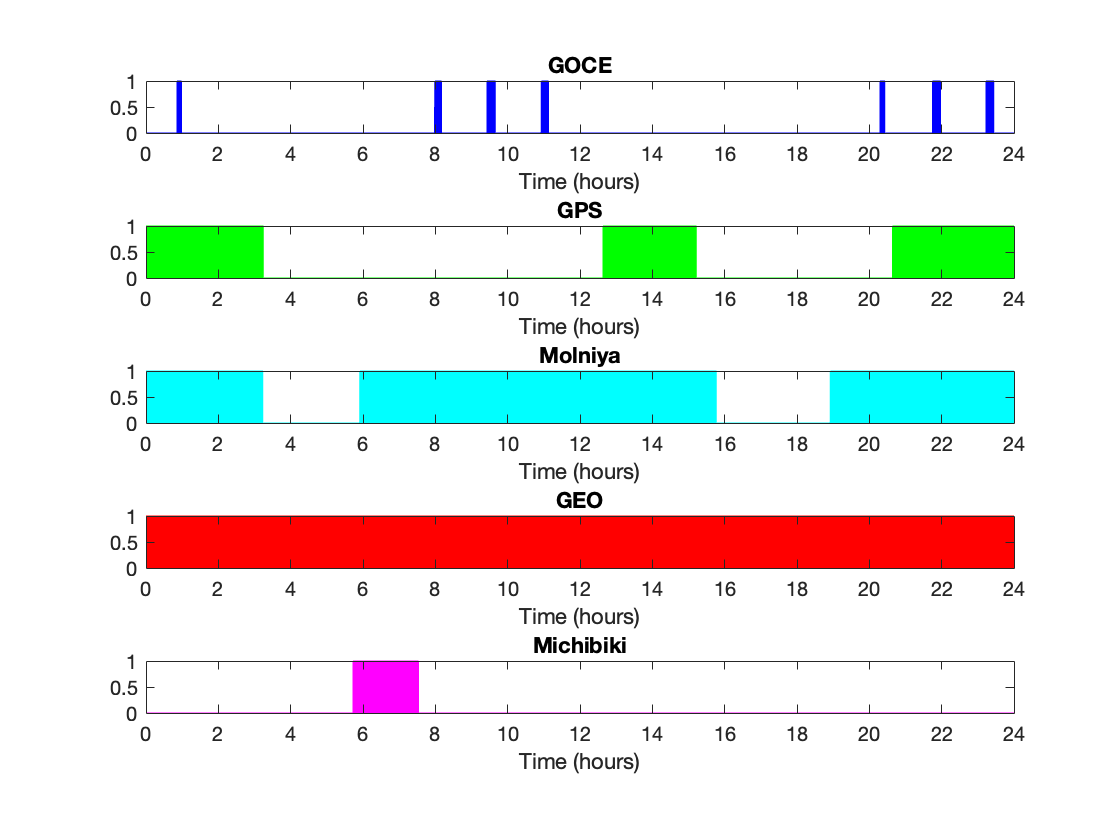
\includegraphics[width=0.7\textwidth]{plots/visual.png}
    \caption{Visibility}
    \label{fig:visibility}
\end{figure}
\end{document}